\documentclass[conference,10pt]{IEEEtran}
\usepackage[T1]{fontenc}
\usepackage{amsmath,amssymb}
\usepackage{graphicx}
\usepackage{booktabs}
\usepackage{multirow}
\usepackage{algorithm}
\usepackage{algpseudocode}
\usepackage{url}
\usepackage{cite}

\begin{document}

\title{Random Forests for Multi-Class Cyberattack Prediction:\\
A Comparison with a Classification Tree and\\ $k$-Nearest Neighbours}

\author{\IEEEauthorblockN{Student number: 27677605}
\IEEEauthorblockA{Computer Science Division, Stellenbosch University}}

\maketitle

\begin{abstract}
A random forest was tuned and evaluated for the prediction of nine cyberattack categories and normal traffic in a network traffic data set with severe class imbalance. The random forest was selected because the forest shares the classification tree base learner used in previous work, so that the comparison isolates the effect of ensembling. Tuning was framed as four questions on ensemble size, the size of the random feature subset, tree complexity and imbalance handling, and was carried out on a subsample that was disjoint from the evaluation data. The tuned forest with a class-balanced bootstrap achieved a macro F1 score of 0.581 and a balanced accuracy of 0.666 over ten folds, compared with 0.573 and 0.636 for the class-weighted classification tree and 0.522 and 0.502 for $k$-nearest neighbours. Both improvements over the tree were statistically significant, but small. A post-hoc run showed that the depth limit selected on the subsample transferred poorly to the full training set: without the limit, the standard forest reached the highest macro F1 score of 0.602, while the balanced forest lost rare-class recall. An analysis of the data showed that 40\,400 records shared an identical feature vector with a record of a different class, which placed a hard ceiling on the separability of the Backdoor, Analysis and Denial of Service categories that no ensemble removes.
\end{abstract}

\begin{IEEEkeywords}
ensemble learning, random forest, bagging, class imbalance, intrusion detection
\end{IEEEkeywords}

\section{Introduction}
Network intrusion detection systems label traffic as normal or as one of several attack types. The labelling task is a multi-class classification problem in which the classes of greatest interest are often the rarest. A previous study on the same network traffic data set compared a single classification tree with $k$-nearest neighbours ($k$NN). The tree achieved the higher macro F1 score, but recall on the rare Backdoor, Analysis and Worms categories remained low.

A single classification tree is an unstable learner. Small changes to the training set produce very different trees, so the predictions of a single tree carry high variance \cite{breiman1996bagging}. Ensemble methods reduce that variance by combining many diverse models \cite{dietterich2000ensemble}. The present study investigated whether an ensemble of trees improves on the single tree and on $k$NN, and why the improvement is as large or as small as observed.

A random forest \cite{breiman2001random} was chosen as the ensemble method. The choice was deliberate. A random forest is built from the same classification and regression tree (CART) learner \cite{breiman1984cart} as the tree in the previous study, so any change in performance is attributable to bagging, random feature selection and voting, and not to a change of base learner. The $k$NN model provides a comparison with a dissimilar, instance-based method.

Tuning was driven by four questions fixed before evaluation:
\begin{enumerate}
\item How many trees are needed before performance stops improving?
\item How does the size of the random feature subset trade the strength of individual trees against diversity between trees, and does random feature selection add value over plain bagging?
\item Do fully grown trees remain the best choice inside an ensemble?
\item Which imbalance remedy gives the best trade-off between macro F1 and recall on rare attack categories?
\end{enumerate}

The remainder of the report is organised as follows. Section~\ref{sec:background} covers the data set, the two baseline models, ensemble learning and the performance measures. Section~\ref{sec:impl} describes the implementation. Section~\ref{sec:emp} sets out the empirical process. Section~\ref{sec:results} presents and discusses the results, and Section~\ref{sec:concl} concludes.

\section{Background}\label{sec:background}

\subsection{The network traffic data set}
The data set is the UNSW-NB15 data set \cite{moustafa2015unsw}, which contains 257\,673 records of network flows. Each record is described by 42 features: three nominal features (protocol, connection state and service) and 39 numeric features that summarise packet counts, byte counts, timing, time-to-live values and connection statistics. The target feature assigns each record to normal traffic or to one of nine attack categories. Table~\ref{tab:data} lists the class distribution. The largest class (Normal) is 534 times larger than the smallest class (Worms).

Moustafa and Slay \cite{moustafa2016evaluation} reported that several attack categories overlap heavily in feature space. The present study quantified that overlap directly: 119\,701 records (46.5\%) share a feature vector with at least one other record, and 40\,400 records share a feature vector with a record that carries a different label. Table~\ref{tab:data} gives the fraction of each class that falls in such conflicting groups. An oracle that memorises the majority label of every distinct feature vector reaches an accuracy of only 0.914 and a macro F1 score of 0.777 on the full data set, because no deterministic function of the features separates identical vectors with different labels. The oracle is an optimistic bound, since the oracle has seen every record. Table~\ref{tab:data} shows that the bound on recall is severe for Backdoor (0.154), Analysis (0.230) and Denial of Service, abbreviated here as DoS (0.544).

\begin{table}[t]
\centering
\caption{Class distribution and label conflicts. ``Conflict'' is the percentage of records whose feature vector also occurs with a different label. ``Oracle'' is the recall of a majority-label lookup on identical vectors.}
\label{tab:data}
\begin{tabular}{lrrrr}
\toprule
Class & Records & \% & Conflict & Oracle \\
\midrule
Normal & 93\,000 & 36.09 & 1.0 & 0.998 \\
Generic & 58\,871 & 22.85 & 0.6 & 0.994 \\
Exploits & 44\,525 & 17.28 & 37.1 & 0.893 \\
Fuzzers & 24\,246 & 9.41 & 14.9 & 0.869 \\
DoS & 16\,353 & 6.35 & 77.4 & 0.544 \\
Reconnaissance & 13\,987 & 5.43 & 16.1 & 0.845 \\
Analysis & 2\,677 & 1.04 & 77.0 & 0.230 \\
Backdoor & 2\,329 & 0.90 & 84.9 & 0.154 \\
Shellcode & 1\,511 & 0.59 & 0.9 & 0.997 \\
Worms & 174 & 0.07 & 8.6 & 0.948 \\
\bottomrule
\end{tabular}
\end{table}

\subsection{Classification trees}
A classification tree recursively partitions the feature space with axis-parallel splits \cite{breiman1984cart}. At each node, CART selects the feature and threshold that maximise the decrease in impurity of the two child nodes. Two impurity measures were considered. The Gini index of a node with class proportions $p_1,\dots,p_K$ is $G = 1-\sum_{c} p_c^2$, and the entropy is $H = -\sum_c p_c \log_2 p_c$. Growth stops when a node is pure, when the tree reaches a maximum depth, or when a split would leave fewer than a minimum number of instances in a leaf. A leaf predicts the class with the largest (weighted) proportion of training instances.

Trees are insensitive to monotone transformations of numeric features, handle mixed feature types, and are easy to interpret. A fully grown tree has low bias but high variance, because each split depends on a small, noisy subset of the data deep in the tree \cite{hastie2009elements}. Class weights multiply the contribution of each instance to the impurity computation, so that a rare class carries as much total weight as a common class.

\subsection{$k$-nearest neighbours}
$k$NN stores the training set and predicts the label of a new instance from the labels of the $k$ closest training instances under a distance metric \cite{cover1967nearest}. With distance weighting, each neighbour votes with a weight inversely proportional to the distance to the query. $k$NN has no training phase, but prediction requires a search over the training set. The method is sensitive to the scale of each feature, so features must be transformed to comparable ranges, and the method suffers when many features are irrelevant or redundant.

\subsection{Ensemble learning}
An ensemble combines the predictions of several base learners. Ensembles outperform members when members are individually accurate and make different errors \cite{dietterich2000ensemble}. For regression with squared error, Krogh and Vedelsby \cite{krogh1995neural} showed that the ensemble error equals the mean member error minus the mean ambiguity (the spread of member predictions around the ensemble prediction). Diversity therefore reduces error only to the extent that strength is not sacrificed. Kuncheva and Whitaker \cite{kuncheva2003measures} reviewed measures of diversity for classifiers, of which the pairwise disagreement (the fraction of instances on which two members predict different labels) is the simplest.

Ensemble methods differ in how members are made diverse. \emph{Bagging} \cite{breiman1996bagging} trains each member on a bootstrap sample of the training set and averages the predictions. Bagging mainly reduces variance and works best for unstable learners such as unpruned trees. \emph{Boosting} \cite{freund1997decision,friedman2001greedy} trains members sequentially, each focused on the errors of the previous members. Boosting mainly reduces bias and is usually applied to shallow trees. \emph{Random subspace} methods \cite{ho1998random} train each member on a random subset of the features.

\subsection{Random forests}
A random forest \cite{breiman2001random} combines bagging with random feature selection at every split. Each tree is grown on a bootstrap sample, and at each node only a random subset of $m$ of the $p$ features is considered for the split. Trees are usually grown to full depth and the forest predicts by majority vote or by averaging class probabilities. Breiman \cite{breiman2001random} bounded the generalisation error of a forest by $\bar\rho(1-s^2)/s^2$, where $s$ is the strength of the individual trees and $\bar\rho$ the mean correlation between trees. A small $m$ decorrelates the trees but weakens each tree, while $m=p$ reduces the forest to bagged trees. The default for classification is $m=\lfloor\sqrt{p}\rfloor$, but Probst \emph{and colleagues} \cite{probst2019hyperparameters} showed that $m$ is the most influential hyperparameter of the forest and that tuning $m$ is worthwhile. The number of trees is not a tuning parameter in the usual sense, since more trees never increase the expected error, but returns diminish quickly \cite{probst2019hyperparameters}.

Each tree leaves out about 36.8\% of the training instances from the bootstrap sample of the tree. Predictions on these out-of-bag instances give an internal estimate of generalisation performance at no extra cost \cite{breiman2001random}.

\subsection{Imbalanced classes in random forests}
Learners that minimise overall error favour the majority classes \cite{he2009learning}. Chen, Liaw and Breiman \cite{chen2004using} proposed two remedies for random forests. A \emph{weighted} random forest assigns class weights in the impurity computation and in the leaf vote. A \emph{balanced} random forest draws each bootstrap sample with the same number of instances from every class, which oversamples rare classes (with replacement) and undersamples common classes. Because every tree sees a different random sample of the majority classes, little information is lost across the forest.

\subsection{Performance measures}
Accuracy is dominated by the large Normal and Generic classes. The macro F1 score is the unweighted mean of the per-class F1 scores, where the F1 score of a class is the harmonic mean of the precision and recall on that class. Macro F1 treats every class equally and was the primary measure, as in the previous study. Balanced accuracy, the unweighted mean of per-class recall, rewards the detection of rare classes regardless of the false alarms produced. The weighted F1 score weights each class by support and was reported for completeness.

\section{Implementation}\label{sec:impl}

\subsection{Data preparation}
Data preparation was identical to the previous study, so that all three models received the same information. The record identifier was removed. Missing service values (54\% of records, marked as ``?'') were kept as a separate level, because a missing service indicates that no known application protocol was used. An ablation in the previous study confirmed that this treatment outperformed mode imputation and removal of the feature. Levels of the nominal features that occur in fewer than 0.1\% of records were merged into a single ``other'' level, which reduced the protocol feature from 133 to 11 levels. The nominal features were one-hot encoded, which gave 64 input features for the tree-based models.

No numeric transformation was applied for the tree and the forest, because a tree split depends only on the order of feature values. For $k$NN, four numeric features with a pairwise correlation above 0.98 with a retained feature were removed, the heavy-tailed numeric features were transformed with $\log(1+x)$, and every feature was scaled to $[0,1]$ with minimum and maximum values computed on the training folds only.

The forest could use the nominal features either as one-hot indicators or as integer codes. Integer codes impose an arbitrary order but keep each nominal feature in a single column, which raises the chance that the feature enters the random subset at a split. The choice was tested empirically (Section~\ref{sec:res-tuning}).

\subsection{Random forest}
The source code is available at \url{https://github.com/hendrikoosthzn/unsw-nb15-ensemble-assignment4}. The forest was implemented in Python on top of the CART implementation of scikit-learn \cite{pedregosa2011scikit}, which was also the implementation of the single tree. The bootstrap, class weighting, random feature selection per split, voting and out-of-bag estimate were implemented explicitly, as summarised in Algorithm~\ref{alg:rf}. A bootstrap sample was represented as a vector of integer multiplicities over the training set and passed to the tree as instance weights. The representation is equivalent to training on the resampled data, but avoids a copy of the data for each tree. Three bootstrap schemes were supported. The standard scheme draws $n$ indices uniformly with replacement. The balanced scheme draws $\lfloor n/K\rfloor$ indices with replacement from each of the $K$ classes. For class weighting, the weight of class $c$ was $n/(K n_c)$, computed either on the full training set or on each bootstrap sample. The forest predicted the class with the largest mean class probability over all trees (soft voting). Trees were trained in parallel threads. To validate the implementation, the forest was compared with the scikit-learn random forest on two folds of the tuning data with identical settings, and the macro F1 scores differed by less than 0.006, which is within the variation caused by the random seed.

\begin{algorithm}[t]
\caption{Random forest training and prediction}\label{alg:rf}
\begin{algorithmic}[1]
\Require training set $\{(\mathbf{x}_i,y_i)\}_{i=1}^n$, trees $T$, features per split $m$, depth limit $d$, minimum leaf size $l$, bootstrap scheme, class weights
\For{$t=1$ \textbf{to} $T$}
\State draw multiplicities $\mathbf{b}^{(t)}\in\mathbb{N}^n$ (standard or balanced bootstrap)
\State $w_i \gets b_i^{(t)}\cdot \omega_{y_i}$ \Comment{class weight $\omega_c=1$ if none}
\State grow CART tree $h_t$ with instance weights $\mathbf{w}$, considering $m$ random features at each split, limited by $d$ and $l$
\State record out-of-bag set $\{i : b_i^{(t)}=0\}$
\EndFor
\State \textbf{predict} $\hat{y}(\mathbf{x})=\arg\max_c \frac{1}{T}\sum_{t=1}^T P_{h_t}(c\mid\mathbf{x})$
\end{algorithmic}
\end{algorithm}

Two diagnostics were computed on the validation fold to address the second tuning question. The \emph{strength} was the mean macro F1 score of the individual trees. The \emph{diversity} was the mean pairwise disagreement over 300 randomly selected pairs of trees.

\subsection{Baseline models}
The classification tree and $k$NN used the final configurations of the previous study. The tree used the Gini index, a maximum depth of 20, a minimum leaf size of one, and balanced class weights. The class weights lowered accuracy but improved recall on the rare classes, which was judged the more important outcome for intrusion detection. $k$NN used $k=7$ with distance weighting and the Euclidean distance on the scaled features. Both configurations had been selected with cross-validation on the same 40\,000-record subsample that was used for tuning in the present study.

\section{Empirical Process}\label{sec:emp}

\subsection{Data partitioning}
The data set was split into two disjoint parts with stratified sampling and a fixed seed. The \emph{tuning set} of 40\,000 records was the same subsample on which the baseline models had been tuned. The \emph{evaluation set} held the remaining 217\,673 records and was not used for any tuning decision in either study. The split removed the optimistic bias of tuning and evaluating on the same records.

\subsection{Tuning}
All tuning experiments used stratified five-fold cross-validation on the tuning set, so that each forest was trained on 32\,000 records. The experiments were run in sequence, each fixing the decisions of the previous experiment:
\begin{itemize}
\item \textbf{E0, encoding:} one-hot indicators against integer codes for the nominal features, with 200 trees and $m=8$ ($\lfloor\sqrt{64}\rfloor$).
\item \textbf{E1, ensemble size:} forests of 500 trees, evaluated on the first $T$ trees for $T$ from one to 500, for $m=8$ and for $m=64$ (bagging).
\item \textbf{E2, features per split:} $m\in\{1,2,4,8,16,32,64\}$ with 200 trees, with strength and diversity recorded.
\item \textbf{E3, tree complexity:} maximum depth in $\{8,12,16,20,24,\text{none}\}$ crossed with minimum leaf size in $\{1,3,10\}$ for the Gini index, and the same depths with a leaf size of one for entropy.
\item \textbf{E4, imbalance:} no remedy, class weights computed on the training set, class weights computed per bootstrap sample, and the balanced bootstrap.
\end{itemize}
Because many settings in E2 and E3 performed similarly, a one-standard-error rule \cite{breiman1984cart} was used to select among settings. The selected setting was the least complex setting whose mean macro F1 score lay within one standard error ($s/\sqrt{5}$ over the five folds) of the best mean. For E4, the selection criterion was macro F1, with balanced accuracy and rare-class recall used to judge the trade-off.

\subsection{Final evaluation}
The final comparison used stratified ten-fold cross-validation on the evaluation set, so that each model was trained on about 195\,900 records and tested on about 21\,800 records per fold. All models were trained and tested on identical folds, which made the fold scores paired. Two forest configurations were evaluated, both with the settings selected in E0 to E3: a forest with the standard bootstrap (RF) and a forest with the balanced bootstrap (RF-B). The second forest was included because the baseline tree used class weights, and a fair test of ensembling required a forest with a comparable imbalance remedy.

For each measure, the Friedman test \cite{friedman1937use} was applied to the four models over the ten folds, followed by pairwise two-sided Wilcoxon signed-rank tests \cite{wilcoxon1945individual} with the Holm correction \cite{holm1979simple} for six comparisons, as recommended by Dem\v{s}ar \cite{demsar2006statistical}. With ten paired folds, the smallest attainable Wilcoxon $p$-value is 0.002, so the smallest attainable corrected $p$-value is 0.012. A significance level of 0.05 was used. Training and prediction times were recorded on a laptop with the same number of threads for all models.

\section{Results and Discussion}\label{sec:results}

\subsection{Tuning results}\label{sec:res-tuning}

\paragraph*{Encoding (E0)} One-hot encoding achieved a mean macro F1 score of 0.516 ($\pm$0.002) against 0.512 ($\pm$0.004) for integer codes. The difference was small, but consistent with the expectation that an arbitrary integer order forces several splits to isolate a single protocol or service level. One-hot encoding was retained, which also kept the input identical to that of the baseline tree.

\paragraph*{Ensemble size (E1)} Figure~\ref{fig:size} shows the macro F1 score against the number of trees. A single bootstrap tree with $m=8$ achieved 0.461, and the score rose steeply up to about 30 trees and levelled off between 50 and 75 trees at about 0.515. Two trees performed worse than one tree, because a tie between two disagreeing trees was resolved in favour of the class with the lowest index, which is Normal. Beyond 75 trees, the changes were smaller than the standard deviation over folds. Bagged trees ($m=64$) followed the same pattern at a slightly higher level. A size of 200 trees was fixed for all further experiments, which left a wide margin above the point of saturation at a modest cost. The result answered the first tuning question: about 50 to 75 trees sufficed, and ensembling raised the macro F1 score of a single bootstrap tree by about 0.05.

\begin{figure}[t]
\centering
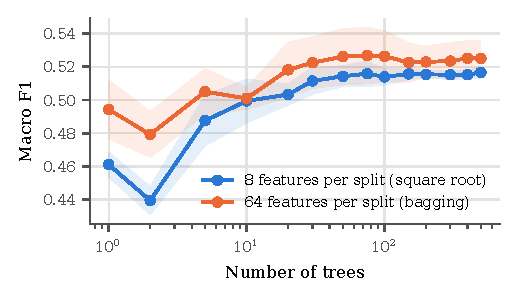
\includegraphics[width=\columnwidth]{figures/size.pdf}
\caption{Macro F1 score against the number of trees on the tuning set (mean over five folds, shaded band one standard deviation).}
\label{fig:size}
\end{figure}

\paragraph*{Features per split (E2)} Figure~\ref{fig:mf} shows the strength--diversity trade-off. As $m$ increased from one to 64, the strength of the individual trees rose from 0.446 to 0.484, and the pairwise disagreement fell from 0.223 to 0.187. The behaviour matched the theory of Breiman \cite{breiman2001random}. However, the macro F1 score of the forest rose with $m$ and then levelled off: 0.494 at $m=1$, 0.516 at $m=8$, 0.521 at $m=16$, and 0.523 for bagging at $m=64$. The gain in strength therefore outweighed the loss of diversity over the whole range, and random feature selection added little over plain bagging on the data set.

A likely explanation is the concentration of predictive information in a few features. The feature importance analysis (Section~\ref{sec:importance}) showed that source bytes, mean source packet size, time-to-live and service carry most of the information. When $m$ is small, most splits must choose among weak features, so trees grow deep without separating the rare classes. Pairwise disagreement remained high even for bagging (0.187), because fully grown trees on bootstrap samples already differ substantially on the overlapping classes. The bootstrap alone therefore supplied enough diversity.

Under the one-standard-error rule, the best mean (0.523 at $m=64$, standard error 0.004) set a threshold of 0.519, and the smallest qualifying value was $m=16$. The value of $m=16$ was selected, which halved the training time of bagging ($8.9$ against $31.0$ seconds per forest).

\begin{figure}[t]
\centering
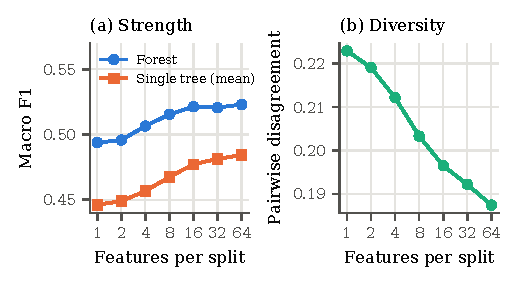
\includegraphics[width=\columnwidth]{figures/max_features.pdf}
\caption{Effect of the number of features considered per split. (a) Macro F1 score of the forest and mean macro F1 score of the individual trees. (b) Mean pairwise disagreement between trees.}
\label{fig:mf}
\end{figure}

\paragraph*{Tree complexity (E3)} Figure~\ref{fig:depth} shows the effect of depth and leaf size. Depth had a strong effect up to a depth of 16: the forest with a depth of eight achieved only 0.427, compared with 0.516 at a depth of 16 (Gini, leaf size one). Beyond a depth of 16, all curves were flat within the noise. At depths of 12 and above, a minimum leaf size of ten reduced the macro F1 score by 0.022 to 0.026, because a leaf of ten instances cannot represent a class such as Worms, which had only about 22 instances in each training fold of the tuning set. Entropy produced slightly higher scores than the Gini index at depths of 16 and above, although the differences were within one standard deviation. The best mean was 0.529 (entropy, depth 24). Under the one-standard-error rule (threshold 0.524), entropy at depths 16, 20 and 24 qualified, and entropy with a depth of 16 and a leaf size of one was selected as the least complex setting. The answer to the third tuning question was therefore that depth must be large, that leaves must be small, and that a depth limit beyond 16 made no measurable difference on 32\,000 training records. Section~\ref{sec:posthoc} revisits the depth limit on the full evaluation set.

\begin{figure}[t]
\centering
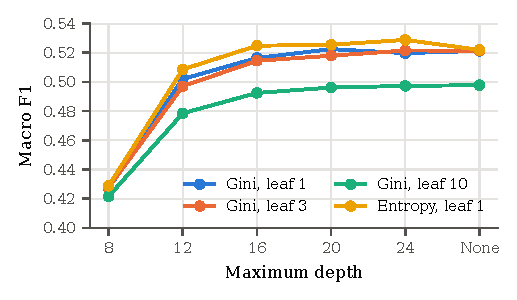
\includegraphics[width=\columnwidth]{figures/depth.pdf}
\caption{Macro F1 score against the maximum tree depth for different minimum leaf sizes and impurity measures ($m=16$, 200 trees).}
\label{fig:depth}
\end{figure}

\paragraph*{Imbalance (E4)} Table~\ref{tab:e4} and Figure~\ref{fig:imb} compare the imbalance remedies. All three remedies improved both macro F1 and balanced accuracy over the unweighted forest. Class weights raised balanced accuracy from 0.509 to 0.557. Weights computed per bootstrap sample performed almost identically to weights computed on the full training set, which was expected, because a bootstrap sample of 32\,000 records preserves the class proportions closely. The balanced bootstrap achieved the highest macro F1 (0.543) and by far the highest balanced accuracy (0.591). Recall on Worms rose from 0.04 to 0.23, on Analysis from 0.06 to 0.26, and on Shellcode from 0.61 to 0.77.

The gains were not free. Recall on Normal fell from 0.94 to 0.79 and recall on Exploits from 0.82 to 0.58, which lowered accuracy from 0.819 to 0.768. For intrusion detection, a lower Normal recall translates into more false alarms. Precision on Normal rose to 0.98, however, so that fewer attacks were labelled as normal traffic, which is the more costly error. The balanced bootstrap differs from class weighting in that each tree sees a balanced sample. With weights, a rare-class instance appears in only about 63\% of the trees and carries a large weight in a few leaves, while with the balanced bootstrap, rare-class instances appear in almost every tree. The balanced bootstrap was selected as the answer to the fourth tuning question.

\begin{table}[t]
\centering
\caption{Imbalance remedies on the tuning set (mean $\pm$ standard deviation over five folds).}
\label{tab:e4}
\setlength{\tabcolsep}{2pt}\footnotesize
\begin{tabular}{lccc}
\toprule
Remedy & Macro F1 & Balanced accuracy & Accuracy \\
\midrule
None & 0.525 $\pm$ 0.013 & 0.509 $\pm$ 0.013 & 0.819 $\pm$ 0.003 \\
Class weights & 0.537 $\pm$ 0.016 & 0.557 $\pm$ 0.011 & 0.789 $\pm$ 0.004 \\
Per-bootstrap weights & 0.542 $\pm$ 0.013 & 0.560 $\pm$ 0.010 & 0.789 $\pm$ 0.005 \\
Balanced bootstrap & \textbf{0.543} $\pm$ 0.024 & \textbf{0.591} $\pm$ 0.020 & 0.768 $\pm$ 0.003 \\
\bottomrule
\end{tabular}
\end{table}

\begin{figure}[t]
\centering
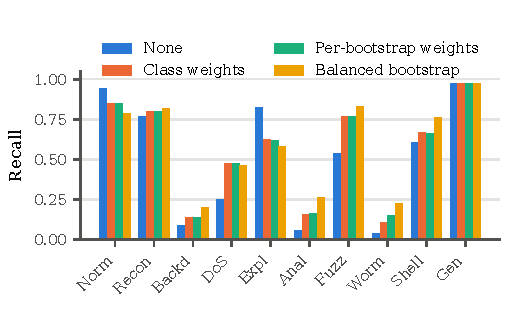
\includegraphics[width=\columnwidth]{figures/imbalance.pdf}
\caption{Per-class recall of the forest under four imbalance remedies on the tuning set.}
\label{fig:imb}
\end{figure}

\subsection{Comparison with the baseline models}
Table~\ref{tab:final} summarises the ten-fold results on the evaluation set, and Table~\ref{tab:tests} reports the statistical tests. The Friedman test rejected the hypothesis of equal performance for macro F1 ($\chi^2=20.5$, $p<0.001$), balanced accuracy ($\chi^2=30.0$, $p<0.001$) and accuracy ($\chi^2=27.1$, $p<0.001$).

\begin{table*}[t]
\centering
\caption{Final evaluation on the 217\,673-record evaluation set (mean $\pm$ standard deviation over ten folds). Times are per fold in seconds.}
\label{tab:final}
\begin{tabular}{lcccccc}
\toprule
Model & Macro F1 & Balanced accuracy & Accuracy & Weighted F1 & Training time & Prediction time \\
\midrule
CART (class weights) & 0.573 $\pm$ 0.013 & 0.636 $\pm$ 0.016 & 0.757 $\pm$ 0.005 & 0.787 $\pm$ 0.004 & 3.1 & 0.004 \\
$k$NN & 0.522 $\pm$ 0.011 & 0.502 $\pm$ 0.009 & 0.805 $\pm$ 0.003 & 0.803 $\pm$ 0.003 & 0.2 & 7.6 \\
RF (standard bootstrap) & 0.572 $\pm$ 0.023 & 0.551 $\pm$ 0.022 & \textbf{0.831} $\pm$ 0.002 & \textbf{0.811} $\pm$ 0.002 & 38.4 & 0.41 \\
RF-B (balanced bootstrap) & \textbf{0.581} $\pm$ 0.011 & \textbf{0.666} $\pm$ 0.016 & 0.757 $\pm$ 0.002 & 0.788 $\pm$ 0.002 & 28.1 & 0.41 \\
\bottomrule
\end{tabular}
\end{table*}

\begin{table}[t]
\centering
\caption{Pairwise Wilcoxon signed-rank tests over ten folds. $\Delta$ is the mean difference (first minus second model), W the number of folds in which the first model scored higher, and $p$ the Holm-corrected $p$-value.}
\label{tab:tests}
\setlength{\tabcolsep}{3.5pt}
\begin{tabular}{lrrrrrr}
\toprule
& \multicolumn{3}{c}{Macro F1} & \multicolumn{3}{c}{Balanced accuracy} \\
\cmidrule(lr){2-4}\cmidrule(lr){5-7}
Comparison & $\Delta$ & W & $p$ & $\Delta$ & W & $p$ \\
\midrule
RF-B against CART & $+$0.008 & 9 & 0.012 & $+$0.030 & 10 & 0.012 \\
RF against CART & $-$0.001 & 6 & 0.984 & $-$0.086 & 0 & 0.012 \\
RF-B against RF & $+$0.009 & 5 & 0.984 & $+$0.115 & 10 & 0.012 \\
CART against $k$NN & $+$0.051 & 10 & 0.012 & $+$0.134 & 10 & 0.012 \\
RF against $k$NN & $+$0.050 & 10 & 0.012 & $+$0.049 & 10 & 0.012 \\
RF-B against $k$NN & $+$0.059 & 10 & 0.012 & $+$0.164 & 10 & 0.012 \\
\bottomrule
\end{tabular}
\end{table}

RF-B achieved the highest macro F1 (0.581) and the highest balanced accuracy (0.666) of all models. RF-B outperformed the class-weighted tree on macro F1 in nine of ten folds and on balanced accuracy in all ten folds, and both differences were significant after correction. The accuracy of RF-B (0.757) was the same as that of the tree. The ensemble therefore improved the detection of rare classes without a further loss of accuracy relative to the single tree, which is consistent with a reduction in the variance of the tree predictions through averaging. The size of the improvement was modest, however: 0.008 in macro F1 and 0.030 in balanced accuracy.

The forest with the standard bootstrap (RF) behaved very differently. RF achieved the highest accuracy (0.831) and weighted F1 (0.811), but the lowest balanced accuracy of the tree-based models (0.551), and RF did not differ significantly from the tree on macro F1. Without an imbalance remedy, RF concentrated on the large classes. RF also showed the largest variation over folds (standard deviation 0.023 in macro F1). The variation came mainly from Worms, with about 15 records per test fold, for which the recall of RF ranged from 0.13 to 0.67 over the folds. The comparison of RF and RF-B shows that, for this data set, the imbalance remedy mattered more than the ensemble itself: the two forests differed by 0.115 in balanced accuracy, while RF-B and the single tree differed by only 0.030.

$k$NN performed worst on macro F1 and balanced accuracy, and was significantly worse than every tree-based model. $k$NN achieved a higher accuracy than the tree (0.805 against 0.757), because $k$NN used no imbalance remedy and favoured the majority classes. The comparison between dissimilar methods therefore favoured the tree family. A plausible reason is that the tree-based models select the few informative features, while $k$NN weights all 60 scaled features equally in the distance computation.

\subsection{Per-class behaviour}
Figure~\ref{fig:perclass} shows the per-class F1 scores and Table~\ref{tab:recall} the per-class recall. The largest gains of RF-B over the tree were on Shellcode (recall 0.79 to 0.93), Fuzzers (0.77 to 0.84), Worms (0.73 to 0.80) and DoS (0.49 to 0.56). On Normal traffic, RF-B had the lowest recall (0.751) but the highest precision (0.992) of all models, so that RF-B rarely labelled an attack as normal traffic but raised more false alarms.

\begin{figure}[t]
\centering
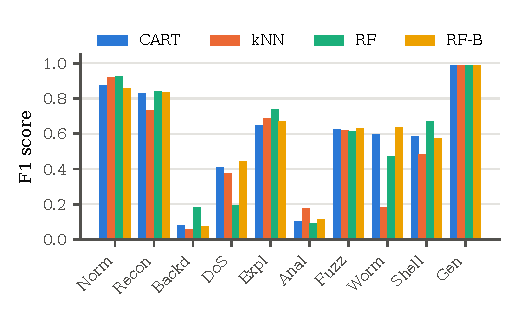
\includegraphics[width=\columnwidth]{figures/perclass_f1.pdf}
\caption{Per-class F1 score on the evaluation set (mean over ten folds).}
\label{fig:perclass}
\end{figure}

\begin{table}[t]
\centering
\caption{Per-class recall on the evaluation set (mean over ten folds), with the oracle bound from Table~\ref{tab:data}.}
\label{tab:recall}
\setlength{\tabcolsep}{4pt}
\begin{tabular}{lccccc}
\toprule
Class & CART & $k$NN & RF & RF-B & Oracle \\
\midrule
Normal & 0.795 & 0.934 & \textbf{0.954} & 0.751 & 0.998 \\
Reconnaissance & 0.799 & 0.723 & 0.766 & \textbf{0.825} & 0.845 \\
Backdoor & \textbf{0.283} & 0.047 & 0.101 & 0.208 & 0.154 \\
DoS & 0.492 & 0.420 & 0.126 & \textbf{0.564} & 0.544 \\
Exploits & 0.516 & 0.706 & \textbf{0.899} & 0.538 & 0.893 \\
Analysis & 0.208 & 0.106 & 0.050 & \textbf{0.230} & 0.230 \\
Fuzzers & 0.767 & 0.558 & 0.546 & \textbf{0.839} & 0.869 \\
Worms & 0.728 & 0.116 & 0.402 & \textbf{0.797} & 0.948 \\
Shellcode & 0.793 & 0.433 & 0.681 & \textbf{0.928} & 0.997 \\
Generic & \textbf{0.982} & 0.978 & \textbf{0.982} & 0.978 & 0.994 \\
\bottomrule
\end{tabular}
\end{table}

Backdoor, Analysis and DoS remained poorly separated by every model. Figure~\ref{fig:cm} shows that the tree and RF-B confused the three categories with one another in almost the same pattern: more than half of the Backdoor records and almost half of the Analysis records were predicted as DoS by RF-B. The label conflict analysis explains the pattern. Between 77\% and 85\% of the records in these categories have a feature vector that also appears with a different label, and the oracle recall is 0.154 for Backdoor and 0.230 for Analysis. The recall of RF-B on Analysis (0.230) and DoS (0.564) already matched or exceeded the oracle, and the higher Backdoor recall of the tree (0.283) came at a precision of only 0.048. The low scores on these categories were therefore a property of the data, not of the models, and no ensemble can remove error that arises from identical inputs with different labels. Ensembling reduces variance, but this error component behaves as irreducible noise. The analysis also explains why the improvement of RF-B over the tree was small: much of the remaining error of the tree lay in the region where improvement was impossible.

\begin{figure*}[t]
\centering
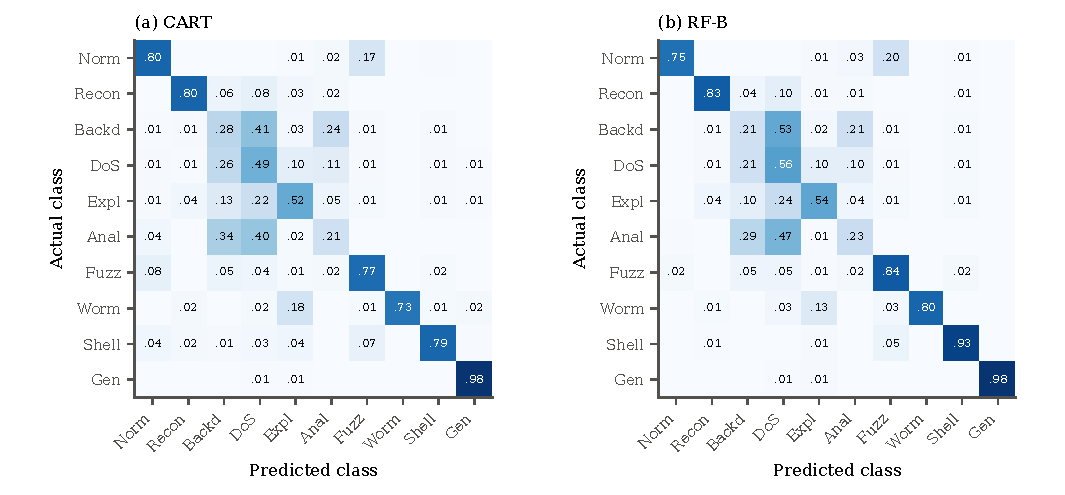
\includegraphics[width=0.85\textwidth]{figures/confusion.pdf}
\caption{Row-normalised confusion matrices on the evaluation set, pooled over ten folds, for (a) the class-weighted classification tree and (b) the forest with the balanced bootstrap. Values below 0.005 are omitted.}
\label{fig:cm}
\end{figure*}

\subsection{Effect of the depth limit on the full data set}\label{sec:posthoc}
The depth limit of 16 was selected on forests trained with 32\,000 records, while the final forests were trained with about 196\,000 records. Because the useful depth of a tree grows with the size of the training set, the selected limit could transfer poorly. A post-hoc run therefore repeated the final evaluation for both forests without a depth limit, with all other settings and the folds unchanged. Table~\ref{tab:posthoc} reports the results. The run used the evaluation set after the main results were known, so the run serves as a diagnostic and not as a tuned result.

\begin{table}[t]
\centering
\caption{Post-hoc effect of removing the depth limit of 16 (mean over ten folds). $\Delta$ is the change relative to the same forest with the depth limit, and W the number of folds in which the unlimited forest scored higher.}
\label{tab:posthoc}
\setlength{\tabcolsep}{3pt}
\begin{tabular}{lcccc}
\toprule
& \multicolumn{2}{c}{RF, no limit} & \multicolumn{2}{c}{RF-B, no limit} \\
\cmidrule(lr){2-3}\cmidrule(lr){4-5}
Measure & Mean & $\Delta$ (W) & Mean & $\Delta$ (W) \\
\midrule
Macro F1 & \textbf{0.602} & $+$0.031 (10) & 0.587 & $+$0.007 (8) \\
Balanced accuracy & 0.578 & $+$0.027 (10) & 0.618 & $-$0.048 (0) \\
Accuracy & \textbf{0.832} & $+$0.001 (8) & 0.773 & $+$0.016 (10) \\
DoS recall & 0.250 & $+$0.124 & 0.267 & $-$0.297 \\
Worms recall & 0.482 & $+$0.080 & 0.757 & $-$0.040 \\
\bottomrule
\end{tabular}
\end{table}

For the forest with the standard bootstrap, removal of the depth limit raised the macro F1 score from 0.572 to 0.602 and balanced accuracy from 0.551 to 0.578, with an improvement in every fold (Holm-corrected Wilcoxon $p=0.008$ for both measures). The unlimited forest achieved the highest macro F1 score of all models and outperformed the class-weighted tree by 0.030 in every fold ($p=0.008$). The depth limit therefore cost the standard forest a substantial part of the benefit of ensembling. On the tuning subsample, unlimited trees (entropy) reached a mean depth of 36 with about 3\,100 leaves, against about 1\,600 leaves at a depth of 16, but the additional leaves did not improve validation performance. With six times as many training records, the deeper splits were supported by enough instances to generalise, particularly for the rare classes.

The balanced forest behaved in the opposite way. Without the depth limit, the macro F1 score rose slightly (0.581 to 0.587, $p=0.027$), but balanced accuracy fell from 0.666 to 0.618 in every fold ($p=0.008$), and DoS recall fell from 0.564 to 0.267. In a balanced bootstrap, each rare-class instance is replicated many times. A fully grown tree isolates these replicated instances in small, pure leaves, so that the forest predicts a rare class only very close to the training instances. A depth limit forces larger leaves that cover a wider region around the rare-class instances, which raises recall on the rare classes at the cost of precision on the common classes. The depth limit therefore acted as a regulariser that interacted with the imbalance remedy.

The post-hoc results refined the answer to the third tuning question. Full depth remained the better choice for the standard forest, as Breiman \cite{breiman2001random} recommended, and the conclusion drawn from the tuning subsample did not transfer to the larger training set. For the balanced forest, the depth limit was beneficial for rare-class recall. Capacity parameters such as depth should therefore be tuned on training sets of the size used in deployment, or expressed relative to the size of the training set. The choice of configuration depends on the objective: the unlimited standard forest maximised macro F1 and accuracy, while the limited balanced forest maximised the detection of rare attacks.

\subsection{Feature importance}\label{sec:importance}
Figure~\ref{fig:imp} shows the mean decrease in impurity of the twelve most important features for RF-B. Source bytes (sbytes) dominated, followed by the mean source packet size (smean), the absence of a known service, the DNS service, the number of connections between the same source and destination (ct\_dst\_src\_ltm) and the source time-to-live (sttl). Six features accounted for 45\% of the total importance, which supports the explanation in E2 that random feature selection with small $m$ forces many splits onto uninformative features. The mean decrease in impurity is biased towards continuous features with many distinct values \cite{strobl2007bias}, so the ranking of the one-hot service indicators is, if anything, understated.

\begin{figure}[t]
\centering
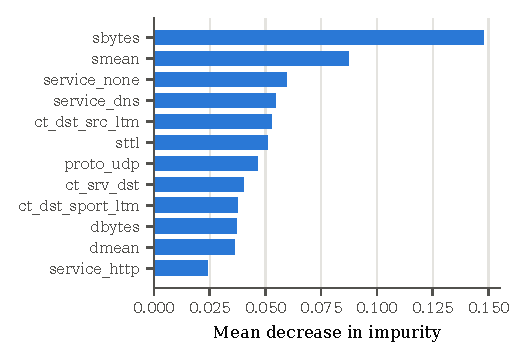
\includegraphics[width=\columnwidth]{figures/importance.pdf}
\caption{Mean decrease in impurity of the twelve most important features for RF-B (mean over ten folds).}
\label{fig:imp}
\end{figure}

\subsection{Computational cost}
The forests were the most expensive models to train: 28 to 38 seconds per fold with the depth limit and a median of 35 to 49 seconds without the limit, against three seconds for the tree. Prediction was fast for all tree-based models (0.4 seconds for about 21\,800 records with 200 trees). $k$NN trained instantly but required 7.6 seconds for prediction, almost 20 times slower than the forest, and the cost grows with the size of the training set. The balanced bootstrap trained faster than the standard bootstrap, because the balanced samples contain many repeated minority instances and therefore fewer distinct instances. For deployment in an intrusion detection system, where prediction speed matters more than training time, the forest is the more practical of the two stronger models.

\section{Conclusions}\label{sec:concl}
A random forest was tuned and compared with the classification tree and $k$NN of a previous study for multi-class cyberattack prediction. The four tuning questions were answered as follows. Performance saturated at 50 to 75 trees. Larger feature subsets increased tree strength more than the corresponding loss of diversity reduced forest performance, so random feature selection added little over bagging, and 16 features per split were selected. Trees had to be deep with small leaves, and a post-hoc run showed that the depth limit of 16 selected on the subsample was too restrictive for the standard forest on the full training set, but helped the balanced forest to retain rare-class recall. The class-balanced bootstrap was the most effective imbalance remedy, and was clearly better than class weighting.

The forest with the balanced bootstrap achieved the highest macro F1 score (0.581) and balanced accuracy (0.666), and significantly outperformed the class-weighted tree and $k$NN. Without the depth limit, the standard forest achieved the highest macro F1 score (0.602) and accuracy (0.832), but a lower balanced accuracy than the tree. The improvement over the single tree was small in every configuration. Two findings explained the size of the gain. First, the imbalance remedy had a larger effect than ensembling itself. Second, a large part of the remaining error arose from records with identical features and different labels, concentrated in the Backdoor, Analysis and DoS categories, which no classifier can separate. Future work should tune tree depth on the full training set and should address the label conflicts directly, for example by merging the inseparable categories or by evaluating on de-duplicated data, before more complex ensembles are considered.

\begin{thebibliography}{99}

\bibitem{moustafa2015unsw}
N.~Moustafa and J.~Slay, ``UNSW-NB15: A comprehensive data set for network intrusion detection systems (UNSW-NB15 network data set),'' in \emph{Proc. Military Communications and Information Systems Conf. (MilCIS)}, 2015, pp.~1--6.

\bibitem{moustafa2016evaluation}
N.~Moustafa and J.~Slay, ``The evaluation of network anomaly detection systems: Statistical analysis of the UNSW-NB15 data set and the comparison with the KDD99 data set,'' \emph{Information Security Journal: A Global Perspective}, vol.~25, no.~1--3, pp.~18--31, 2016.

\bibitem{breiman1984cart}
L.~Breiman, J.~H. Friedman, R.~A. Olshen, and C.~J. Stone, \emph{Classification and Regression Trees}. Belmont, CA, USA: Wadsworth, 1984.

\bibitem{cover1967nearest}
T.~M. Cover and P.~E. Hart, ``Nearest neighbor pattern classification,'' \emph{IEEE Transactions on Information Theory}, vol.~13, no.~1, pp.~21--27, 1967.

\bibitem{hastie2009elements}
T.~Hastie, R.~Tibshirani, and J.~Friedman, \emph{The Elements of Statistical Learning}, 2nd~ed. New York, NY, USA: Springer, 2009.

\bibitem{dietterich2000ensemble}
T.~G. Dietterich, ``Ensemble methods in machine learning,'' in \emph{Multiple Classifier Systems}, Lecture Notes in Computer Science, vol.~1857. Berlin, Germany: Springer, 2000, pp.~1--15.

\bibitem{krogh1995neural}
A.~Krogh and J.~Vedelsby, ``Neural network ensembles, cross validation, and active learning,'' in \emph{Advances in Neural Information Processing Systems}, vol.~7, 1995, pp.~231--238.

\bibitem{kuncheva2003measures}
L.~I. Kuncheva and C.~J. Whitaker, ``Measures of diversity in classifier ensembles and their relationship with the ensemble accuracy,'' \emph{Machine Learning}, vol.~51, no.~2, pp.~181--207, 2003.

\bibitem{breiman1996bagging}
L.~Breiman, ``Bagging predictors,'' \emph{Machine Learning}, vol.~24, no.~2, pp.~123--140, 1996.

\bibitem{freund1997decision}
Y.~Freund and R.~E. Schapire, ``A decision-theoretic generalization of on-line learning and an application to boosting,'' \emph{Journal of Computer and System Sciences}, vol.~55, no.~1, pp.~119--139, 1997.

\bibitem{friedman2001greedy}
J.~H. Friedman, ``Greedy function approximation: A gradient boosting machine,'' \emph{The Annals of Statistics}, vol.~29, no.~5, pp.~1189--1232, 2001.

\bibitem{ho1998random}
T.~K. Ho, ``The random subspace method for constructing decision forests,'' \emph{IEEE Transactions on Pattern Analysis and Machine Intelligence}, vol.~20, no.~8, pp.~832--844, 1998.

\bibitem{breiman2001random}
L.~Breiman, ``Random forests,'' \emph{Machine Learning}, vol.~45, no.~1, pp.~5--32, 2001.

\bibitem{probst2019hyperparameters}
P.~Probst, M.~N. Wright, and A.-L. Boulesteix, ``Hyperparameters and tuning strategies for random forest,'' \emph{Wiley Interdisciplinary Reviews: Data Mining and Knowledge Discovery}, vol.~9, no.~3, e1301, 2019.

\bibitem{he2009learning}
H.~He and E.~A. Garcia, ``Learning from imbalanced data,'' \emph{IEEE Transactions on Knowledge and Data Engineering}, vol.~21, no.~9, pp.~1263--1284, 2009.

\bibitem{chen2004using}
C.~Chen, A.~Liaw, and L.~Breiman, ``Using random forest to learn imbalanced data,'' Department of Statistics, University of California, Berkeley, Technical Report 666, 2004.

\bibitem{pedregosa2011scikit}
F.~Pedregosa, G.~Varoquaux, A.~Gramfort, V.~Michel, B.~Thirion, O.~Grisel, M.~Blondel, P.~Prettenhofer, R.~Weiss, V.~Dubourg, J.~Vanderplas, A.~Passos, D.~Cournapeau, M.~Brucher, M.~Perrot, and E.~Duchesnay, ``Scikit-learn: Machine learning in Python,'' \emph{Journal of Machine Learning Research}, vol.~12, pp.~2825--2830, 2011.

\bibitem{friedman1937use}
M.~Friedman, ``The use of ranks to avoid the assumption of normality implicit in the analysis of variance,'' \emph{Journal of the American Statistical Association}, vol.~32, no.~200, pp.~675--701, 1937.

\bibitem{wilcoxon1945individual}
F.~Wilcoxon, ``Individual comparisons by ranking methods,'' \emph{Biometrics Bulletin}, vol.~1, no.~6, pp.~80--83, 1945.

\bibitem{holm1979simple}
S.~Holm, ``A simple sequentially rejective multiple test procedure,'' \emph{Scandinavian Journal of Statistics}, vol.~6, no.~2, pp.~65--70, 1979.

\bibitem{demsar2006statistical}
J.~Dem\v{s}ar, ``Statistical comparisons of classifiers over multiple data sets,'' \emph{Journal of Machine Learning Research}, vol.~7, pp.~1--30, 2006.

\bibitem{strobl2007bias}
C.~Strobl, A.-L. Boulesteix, A.~Zeileis, and T.~Hothorn, ``Bias in random forest variable importance measures: Illustrations, sources and a solution,'' \emph{BMC Bioinformatics}, vol.~8, art.~25, 2007.

\end{thebibliography}

\end{document}
